\label{sec:method}

\section{Method}
The whole architecture of our method is presented in Figure.~\ref{fig:main_figure}. A point cloud video sequence for human instances is denoted as $PC \in 
 \mathcal{R}^{L \times N \times D}$, where $L$ is the sequence length, $N$ is number of points in each frame, and $D$ is the dimension of each point. 
To exploit both the structural semantics of human body and human motion to facilitate the acquisition of human-specific features from sequences of point clouds, we create two large-scale point-cloud-based datasets and corresponding pre-trained networks for body segmentation and motion flow estimation in \textbf{Prior Knowledge Extraction}.
% so that human prior knowledge can be learned in advance and assist subsequent representation learning. 
Besides, to learn the essential geometric and dynamic representations of humans from data itself, we explore the spatial and temporal relationships of structural semantics in human body by applying spatio-temporal modeling upon the embedding of body parts in the stage of \textbf{Semantic-guided Spatio-temporal Representation Self-learning}.
%compared to recent work~\cite{shen2023masked} who establish global relationships among flattened tubes built from FPS sampling and clustering which inadvertently compromises the semantic and dynamic consistency in 4D videos. 
Building upon this foundation, we use extracted multiple levels of human-related prior knowledge to benefit various downstream tasks by \textbf{Hierarchical Feature Enhanced Fine-tuning}, which integrates global-level, part-level, and point-level point cloud features.



\subsection{Prior Knowledge Extraction}
Different from the movements of rigid objects such as vehicles in traffic scenarios, the motion of non-rigid humans is more complicated, for it contains not only global rotations and translations but also local rotations and translations, such as relative motions among joints, making capturing human motion features more challenging. The key to addressing this problem is to model the human motion in more fine-grained levels, including body part level and point-wise level. Therefore, we build the Human Body Segmentation (HBSeg) and Human Motion Flow (HMFlow) networks to provide more fine-grained geometric and motion information about human body, which can serve as prior knowledge to facilitate following human-centric representation learning.
% Therefore, we pre-trained the HMFlow on synthetic data to provide point-wise motion information and benefit the enhancement of the hierarchical features when fine-tuning on downstream tasks.
\subsubsection{Human Body Segmentation (HBSeg)}
\begin{figure}[h]
    \centering  
    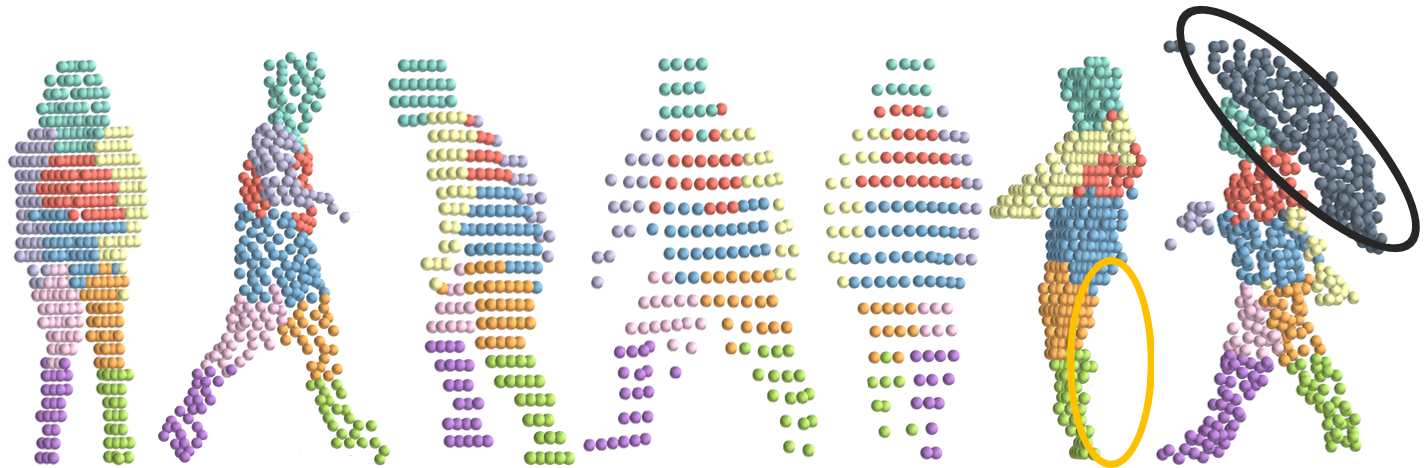
\includegraphics[width=0.5\textwidth]
    {pic/part_black_noise.png} 
    \caption{Visualization results of HBSeg on HuCenLife~\cite{xu2023human}.
    We show cases with different densities of LiDAR point cloud, occlusion (yellow circle), and noise (black circle). HBSeg has robust performance even merely trained on our synthesized dataset.}

    
    
    
    \label{fig:partseg_6.png}
 \end{figure}




\label{subsec:HBPSegModule}
To fully utilize the structural semantics of human body, we deconstruct human into fine-grained body parts by HBSeg, pre-trained on our synthetic dataset, which is constructed by employing a simulated LiDAR model~\cite{ren2023lidar} to scan the surfaces of 3D human meshes from the AMASS dataset~\cite{mahmood2019amass} at various perspectives and distances, meanwhile introducing random occlusions and noise to minimize the distribution gap between synthetic data and real data. We define 9 parts of human body and generate annotations by attaching the body part label of the nearest SMPL~\cite{loper2023smpl} mesh vertex to the synthetic LiDAR Point. More details are in Section.~\ref{subsubsec:HBPSegData} and supplementary material.

We adopt the PointNeXt-L~\cite{qian2022pointnext} as the main body network of HBSeg. 
After training on synthetic data, we apply the pre-trained HBSeg on real data to get the part segmentation labels $S \in \mathcal{R}^{L \times N \times 1}$. As Figure.~\ref{fig:partseg_6.png} shows, HBSeg performs stable on real-life data with changing sparsity and works well even for occlusion and noise cases, mainly due to our efforts on generating realistic synthetic data.
%For missing parts, we use information from adjacent frames to complete them.
% \begin{figure*}[t]
%     \centering
%     \includegraphics[width=2.2\columnwidth]{pic/part_seg.drawio.pdf}
%     \caption{Visualization of Human Body Part Segmentation(HBPSeg) geometric
%      }
%     \label{fig:vis_HBPSeg}
%     \vspace{-1ex}
% \end{figure*}


\subsubsection{Human Motion Flow Estimation (HMFlow)}



\begin{figure}[h]
    \centering  
    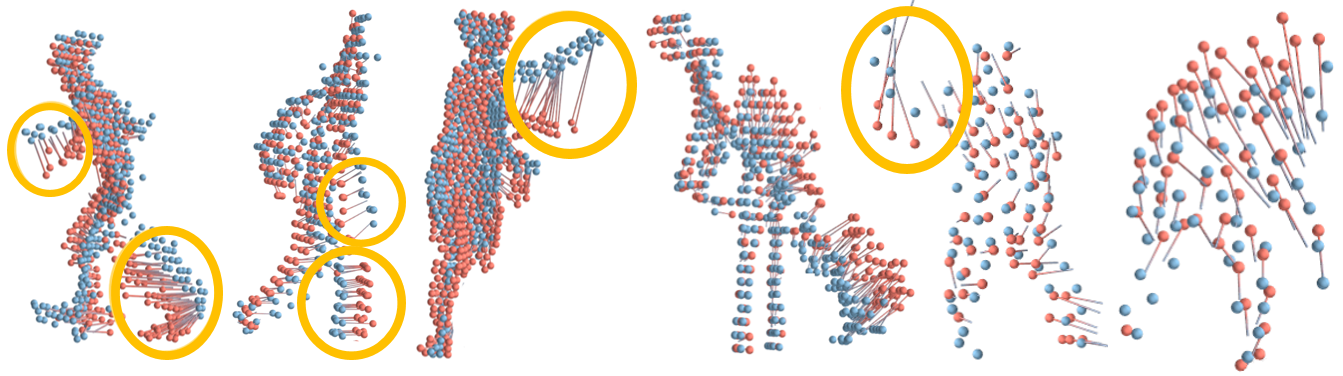
\includegraphics[width=0.46\textwidth]{pic/motion_sorted.png}  
    \caption{Visualization results of HMFlow on HuCenLife~\cite{xu2023human}. We present several cases from near to far relative to the LiDAR sensor. HMFlow has good capability of estimating point flow even for the parts with significant movements (yellow circle), which can provide explicit features of human dynamics.}


    % from dense to sparse. Yellow circles represent significant movements of human parts like waving arms and stretching legs. Our motion flow can track the movement, enabling us to better extract dynamic features.
    \label{fig:vis_HMFlow}
 \end{figure}


\label{subsec:HMFlowModule}
% However, most of these works focuses on rigid transformations in scenes. For non-rigid objects like the human body, there exist not only global rotations and translations but also local rotations and translations, such as relative motions among joints, which is more complicated and challenging. To address this problem, we create a synthetic dataset with human motion flow ground truth to train the flow estimator, which can provide point-wise motion information to benefit the motion feature extraction of point cloud humans.
% Different from the movements of rigid objects such as vehicles in traffic scenarios, the motion of non-rigid humans is more complicated, for it contains not only global rotations and translations but also local rotations and translations, such as relative motions among joints, which means capturing human motion features is more challenging. The key to address this problem is to model the human motion in more fine-grained levels, such as body part level or point-wise level. 
We pre-train the HMFlow on our synthetic dataset to provide point-wise motion information, which can benefit the feature enhancement in the fine-tuning stage.
Similar to Section.~\ref{subsec:HBPSegModule}, we associate each synthetic LiDAR point to its nearest SMPL vertex. Therefore, we are able to establish the correspondence between synthetic LiDAR points across different frames by using SMPL vertices indices, so that we can obtain motion flow ground truth for training our HMFlow. More details are in Section.~\ref{subsubsec:HMFlowData} and supplementary material.

We employ FLOT~\cite{puy2020flot} as the human motion flow estimator, which casts the task of scene flow estimation as finding soft correspondences on a pair of point clouds via solving an optimal transport problem~\cite{li2023deep}. When testing on the real data, we input adjacent LiDAR point clouds $PC_t$ and $PC_{t+1} \in \mathcal{R}^{L \times N \times D}$ into the pre-trained HMFlow to obtain human motion flow vectors $F \in \mathcal{R}^{L \times N \times D'}$ for each LiDAR point in the t-th frame. As Figure.~\ref{fig:vis_HMFlow} demonstrates, HMFlow can generate reasonable prediction for point-wise motion flow on real data even without annotations, which is valuable to provide explicit priors for human dynamics.

% The latent features of $F$ will be fused with those of points in our  in the fine-tuning stage, therefore we fully extract the information in point level which contains the point-wise position, motion direction and motion displacement. 
% Finally, we obtain three levels of representation for human-centric LiDAR point cloud videos: global human instance level, local body parts level, and point-wise level. Our model achieve good performance by making full use of information in three levels .


\subsection{Semantic-guided Spatio-temporal Representation Self-learning}
\label{subsec:STMaskRecon}
Due to spatial irregularities and temporal redundancies, annotating dynamic point cloud videos is labor-intensive and error-prone. Moreover, fully-supervised methods usually overfit to manual annotations in specific domains, struggling to capture the underlying patterns of new data~\cite{zeng2023self}. This limitation leads to a restricted ability to generalize to other tasks or datasets. Additionally, existing feature extraction networks employ generic point-cloud-based backbones that are ill-suited for human-centric data, as they do not account for human-specific characteristics.
Based on structure semantics of human bodies obtained in previous stage, we propose a module, named Semantic-guided Spatio-temporal Representation Self-learning, which mines essential geometric and motion features from human point cloud video data itself by masking and predicting body part patches to enhance the generalization ability of the model to benefit a variety of downstream tasks.

As Figure.~\ref{fig:main_figure} shows, We first mask some of the body-part tokens in temporal and spatial dimensions. After extracting the token embedding of part patches, only visible tokens will be input to the STEncoder to extract latent representation, which will be decoded with masked tokens together to reconstruct the 3D Cartesian coordinates of masked part patches. Details are as follows.




\subsubsection{Spatio-temporal Masking Strategy}
In temporal dimension, we mask all part patches in some random frames and reconstruct the masked tokens, encouraging STEncoder networks to estimate the part motion over a long period.
In spatial dimension, we randomly mask some part patches in the remaining frames after temporal masking, making the STEncoder network estimate the spatial geometric features of the entire human based on the visible tokens.

We apply temporal masking first, and then spatial masking. Given part patches $P \in \mathcal{R}^{L \times M \times N' \times D}$, we adopt a temporal mask ratio $r_t$ and spatial mask ratio $r_s$, respectively. Firstly, all part patches in $r_tL$ frames are masked, named as temporal masked patches $P_M^t \in \mathcal{R}^{r_tL \times M \times N' \times D}$, which will be used as the reconstruction ground truth of temporal masking. For every frame of the remaining $(1-r_t)L$ visible frames, $r_sM$ part patches are masked randomly, hence spatial masked patches $P_M^s \in \mathcal{R}^{(1-r_t)L \times r_sM \times N' \times D}$ will be used as the reconstruction ground truth of the spatial masking.

\subsubsection{Embedding Layer}
\label{subsubsec:embedding}
For visible part patches, we use Mini-PointNet~\cite{qi2017pointnet} as a tokenizer to obtain visible part tokens embedding $T_V$ from visible part patches $P_V$. 
\begin{equation}
    \begin{aligned}
    T_V = Tokenizer(P_V),
    \end{aligned}
\end{equation}
where $T_V \in \mathcal{R}^{(1-r_t)L \times (1-r_s)M \times C}$, $P_V \in \mathcal{R}^{(1-r_t)L \times (1-r_s)M \times N' \times D}$. $C$ is the channel dimension of part tokens. 
 % The features of motion flow will only be element-wise added to those of part tokens in fine-tuning stage to prevent the leakage of location information to the STEncoder in pre-trained stage.
For every masked part patch, we replace it with a share-weighted learnable masked part token $T_M$, which will be concatenated with the output of STEncoder and processed by the decoder together.

Learnable spatial positional encoding and temporal positional encoding will also be added to the input of every transformer layer in the STEncoder and decoder. 


\subsubsection{Spatio-temporal Encoder (STEncoder)}

To fully utilize the inherent structure of the human body, characterized by fixed components such as torso, head, arms, and legs, as well as the distinctive dynamic traits exhibited during human motion, our STEncoder applies spatial modeling and temporal modeling on body part tokens, respectively.
The STEncoder learns to extract the high-level latent geometric and motion features of humans from only $T_V$, which are input to STEncoder to get enhanced visible part tokens $T_V^E$.

For the network design of STEncoder, we interlace multiple spatial transformer~\cite{vaswani2017attention} layers and temporal transformer layers to extract the spatial geometry feature and temporal motion feature, respectively. For each spatial transformer layer, we apply self-attention~\cite{vaswani2017attention} among all visible parts tokens in every frame:
\begin{equation}
    \begin{aligned}
    V^{s'}_T = SpatialTransformer(V^{s}_T),
    \end{aligned}
\end{equation}
where $V^{s}_T, V^{s'}_T \in \mathcal{R}^{(1-r_s)M \times C}$ are the visible part tokens in a frame. For each temporal transformer layer, we apply self-attention for every visible part token among all L frames:
\begin{equation}
    \begin{aligned}
    V^{t'}_T = TemporalTransformer(V^{t}_T),
    \end{aligned}
\end{equation}
where $V^{t}_T, V^{t'}_T \in \mathcal{R}^{(1-r_t)L\times C}$ are the visible part tokens of a body part in $L$ frames.

\subsubsection{Mask Reconstruction}
Our decoder is similar to the STEncoder with fewer layers. We take the enhanced visible part tokens $T_V^E$ as well as masked part token $T_M$ as the input of the decoder. 
\begin{equation}
    \begin{aligned}
    T_R = Decoder(Concate(T_V^E,T_M)),
    \end{aligned}
\end{equation}
where $T_R \in \mathcal{R}^{L \times M \times C}$ is reconstructed part tokens.

Among the $T_R$, only the tokens masked before will be fed to the reconstruction head to predict the original masked part patches. The structure of the reconstruction head is similar to that in Point-MAE~\cite{pang2022masked}, which is a fully connected (FC) layer with a reshape operation.
\begin{equation}
    \begin{aligned}
    P^s_R = Reshape(FC(T^s_R)), \\
    P^t_R = Reshape(FC(T^t_R)), 
    \end{aligned}
\end{equation}
where $P^s_R \in \mathcal{R}^{(1-r_t)L \times r_sM \times N' \times D}$, $T^s_R \in \mathcal{R}^{(1-r_t)L \times r_sM \times C}$, $P^t_R \in \mathcal{R}^{r_tL \times M \times N' \times D}$, $T^t_R \in \mathcal{R}^{r_tL \times M \times C}$ are spatial reconstructed part patches, spatial reconstructed part tokens, temporal reconstructed part patches, temporal reconstructed part tokens, respectively.
We first reconstruct the spatial masked tokens, and then the temporal masked tokens. We adopt Chamfer Distance~\cite{fan2017point} Loss $L_{CD}$ as the reconstruction loss function:

\begin{equation}
    \begin{aligned}
    L_{CD} (P_M,P_R) = \frac{1}{\|P_M\|}\sum_{x \in P_M}\min_{y \in P_R}\|x-y\|_{2}^2 \\
    +\frac{1}{\|P_R\|}\sum_{y \in P_R}\min_{x \in P_M}\| y-x \|_{2}^2.
    \end{aligned}
\end{equation}
% where $MP_s \in \mathcal{R}^{(1-r_t)T \times r_sM}$ are Spatial Mask Patches served as the ground truth of spatial reconstruction.
% \begin{equation}
%     \begin{aligned}
%     L^t_{CD} (MP_t,RP_t) = \frac{1}{\|MP_t\|}\sum_{x \in MP_t}\min_{y \in RP_t}\|x-y\|_{2}^2 \\
%     +\frac{1}{\|RP_t\|}\sum_{y \in RP_t}\min_{x \in MP_t}\| y-x \|_{2}^2
%     \end{aligned}
% \end{equation}
% where $MP_t \in \mathcal{R}^{r_tT \times M}$ are Temporal Mask Patches served as the ground truth of temporal reconstruction.

\subsection{Hierarchical Feature Enhanced Fine-tuning}
\label{subsec:finetine}
After the above self-learning process, STEncoder is endowed with the ability to extract the representations of humans in part-level structural semantics. When fine-tuning on multiple downstream tasks, hierarchical features can enhance the STEncoder to capture more complicated and challenging fine-grained geometric and dynamic representations.
Specifically, we integrate global-level, part-level, and point-level point cloud features to pre-trained STEncoder (See Figure.~\ref{fig:main_figure}), therefore fully leveraging prior knowledge for effective and robust human-centric representation learning. 
 

During this stage, all part patches are visible to the STEncoder, and information of point-wise motion flow vector will be fused to that of body parts in Tokenizer. (See details in supplementary materials)
\begin{equation}
    \begin{aligned}
    T = Tokenizer(P,F),
    \end{aligned}
\end{equation}
where $T \in \mathcal{R}^{L \times M \times C}, P \in \mathcal{R}^{L \times M \times N' \times D}, F \in \mathcal{R}^{L \times M \times N' \times D'}$ are part tokens, part patches, and motion flow vectors, respectively. We will also append a global token extracted from the entire human instance to enable the interaction of features between global and part. For classification tasks like action recognition, a class token will be appended as well.
we discard the decoder and add corresponding task heads after the pre-trained tokenizer, learnable position encoding, and STEncoder for different tasks.
